\documentclass[11pt,a4paper]{article}

\usepackage[utf8]{inputenc}
\usepackage[T1]{fontenc}
\usepackage[spanish,es-nodecimaldot]{babel}
\usepackage{lmodern}
\usepackage[a4paper,margin=2.1cm,headheight=14pt,footskip=1.2cm]{geometry}
\usepackage{xcolor}
\usepackage{fancyhdr}
\usepackage{graphicx}
\usepackage{booktabs}
\usepackage{array}
\usepackage[hidelinks]{hyperref}
\usepackage{microtype}

\definecolor{navy}{HTML}{10283F}
\definecolor{teal}{HTML}{147A86}
\setlength{\parindent}{0pt}
\setlength{\parskip}{0.55em}
\sloppy

\pagestyle{fancy}
\fancyhf{}
\renewcommand{\headrulewidth}{0pt}
\renewcommand{\footrulewidth}{0.3pt}
\fancyfoot[L]{\footnotesize UTEC -- CS2023 \textbar{} Proyecto Final 2}
\fancyfoot[R]{\footnotesize Pág. \thepage}

\begin{document}
\thispagestyle{fancy}

\vspace*{1.5cm}
\begin{center}
  {\LARGE\bfseries\color{navy} Proyecto Final 2 -- Anima tu Algoritmo o Estructura de Datos\par}
  \vspace{0.8cm}
  {\Large\bfseries\color{teal} Articulaciones en grafos no dirigidos\par}
\end{center}
\vspace{1.3cm}

\textbf{Universidad:} Universidad de Ingeniería y Tecnología (UTEC)\\[0.25em]
\textbf{Curso:} CS2023 -- Algoritmos y Estructuras de Datos, ciclo 2026-2\\[0.25em]
\textbf{Docente:} Prof. Víctor Racsó Galván Oyola\\[0.25em]
\textbf{Algoritmo asignado:} Detección de articulaciones en grafos no dirigidos

\vspace{0.7cm}
\textbf{Integrantes:}
\begin{itemize}
  \item Huertos Ochoa, Rodrigo Franco
  \item Ramos Vargas, Royer Sebastián
  \item Rosario Palomino, Diego Antonio
\end{itemize}

\vspace{0.5cm}
\textbf{Fecha:} 18 de noviembre de 2026

\newpage

\section*{Resumen}
Se implementó un detector de \textbf{articulaciones} (vértices de corte) en
grafos no dirigidos en C++17 mediante búsqueda en profundidad (DFS) con tiempos
de descubrimiento (\texttt{tin}) y valores \texttt{low}. El programa ejecuta
una lógica propia sin bibliotecas externas de algoritmos de grafos y emite una
traza real en formato JSON (\texttt{trazas.json}). Un pipeline en Python con
Pillow y FFmpeg consume dichas trazas para renderizar un video explicativo de
180 segundos en 1920\,$\times$\,1080, garantizando que cada estado visualizado
corresponda exactamente a la ejecución del motor en C++.

\section{Algoritmo asignado y fundamentos}
Dado un grafo no dirigido $G=(V,E)$, sea $c(G)$ el número de componentes
conexas de $G$. Un vértice $v \in V$ es una \textbf{articulación} si su
eliminación junto con sus aristas incidentes incrementa el número de
componentes conexas:
\[
  c(G - v) > c(G)
\]
Esta definición se mantiene válida tanto en grafos conexos como desconectados.
En redes de comunicación o infraestructura, las articulaciones identifican los
puntos críticos de falla cuya caída fragmentaría la conectividad del sistema.

El algoritmo (\texttt{Solver} en \texttt{implementacion\_cpp/articulaciones.cpp})
recorre cada componente conexa no visitada mediante DFS manteniendo cuatro
arreglos indexados por vértice:
\begin{itemize}
  \item \texttt{tin[v]}: instante en que se descubre el vértice $v$ por primera
    vez (\texttt{-1} si aún no fue visitado).
  \item \texttt{low[v]}: menor tiempo de descubrimiento alcanzable desde $v$ o
    desde su subárbol DFS empleando a lo más una arista de retorno.
  \item \texttt{parent[v]}: padre de $v$ en el árbol DFS.
  \item \texttt{cut[v]}: indicador binario de si $v$ es vértice de corte.
\end{itemize}

Al explorar una arista hacia un vecino \texttt{to}, se ignora únicamente la
arista específica por la cual se descendió desde el padre (identificada por su
índice en \texttt{edges}), lo que permite procesar correctamente lazos y
aristas paralelas:
\begin{enumerate}
  \item Si \texttt{to} ya fue visitado, se actualiza
    $\texttt{low}[v] = \min(\texttt{low}[v], \texttt{tin}[\texttt{to}])$.
  \item Si \texttt{to} no fue visitado, se desciende recursivamente y, al
    retornar, se propaga
    $\texttt{low}[v] = \min(\texttt{low}[v], \texttt{low}[\texttt{to}])$.
    Si $v$ no es raíz y $\texttt{low}[\texttt{to}] \ge \texttt{tin}[v]$, el
    subárbol de \texttt{to} no tiene retorno hacia un ancestro estricto de $v$,
    por lo que $v$ se marca como articulación.
  \item Para la \textbf{raíz del árbol DFS} (\texttt{parentEdge == -1}), se
    aplica la regla específica: es articulación si y solo si posee más de un
    hijo en el árbol DFS (\texttt{children > 1}).
\end{enumerate}

\section{Implementación y herramientas}
\begin{itemize}
  \item \textbf{C++17 (\texttt{g++} / \texttt{clang++} / MSVC):} implementa el
    algoritmo de Tarjan/DFS sobre listas de adyacencia propias usando
    \texttt{std::vector} y el modo \texttt{--trace} para emitir eventos JSON
    (\texttt{discover}, \texttt{tree}, \texttt{back}, \texttt{return},
    \texttt{cut}, \texttt{root}, \texttt{finish} y \texttt{result}).
  \item \textbf{CMake 3.20+ y CTest:} configuración multiplataforma de
    compilación y registro de pruebas automáticas.
  \item \textbf{Python 3.10+ y Pillow (\texttt{>=10.4,<14}):} orquesta la
    compilación, genera \texttt{trazas.json}, verifica coherencia contra un
    oráculo independiente y dibuja cada fotograma a partir de la traza real.
  \item \textbf{FFmpeg y \texttt{ffprobe}:} codifica los fotogramas RGB en
    MP4 (H.264, \texttt{yuv420p}) y, opcionalmente, mezcla una pista de audio
    en AAC mediante \texttt{agregar\_voz.py}.
\end{itemize}

\emph{Nota de transparencia:} El código, los visuales y la redacción técnica
contaron con asistencia de herramientas de IA; todo resultado fue verificado por
el equipo mediante el oráculo independiente y la validación de trazas.

\section{Pasos para reproducir el video}
Desde la raíz del repositorio, configurar el entorno Python e instalar Pillow:
\begin{verbatim}
python -m venv .venv
.\.venv\Scripts\Activate.ps1
python -m pip install -r animacion_python/requirements.txt
\end{verbatim}

Compilar el motor C++, generar las trazas y validar contra el oráculo:
\begin{verbatim}
python animacion_python/proyecto.py --prepare
python implementacion_cpp/tests/test_articulaciones.py
python animacion_python/verify_trace.py
\end{verbatim}

Renderizar el video final (o usar \texttt{--all} para ejecutar todo en un solo paso):
\begin{verbatim}
python animacion_python/proyecto.py --video
\end{verbatim}

Opcionalmente, desde PowerShell puede usarse \texttt{./ejecutar.ps1 -Accion all},
agregar narración sincronizada con \texttt{python animacion\_python/agregar\_voz.py
ruta/voz.wav} y empaquetar el entregable con \texttt{python empaquetar.py}. El
video resultante (\texttt{animacion\_python/output/articulaciones\_sin\_voz.mp4})
tiene una duración de \textbf{180 segundos} (8 escenas), resolución de
\textbf{1920\,$\times$\,1080} y \textbf{24 fotogramas por segundo} (12 estados
dibujados por segundo duplicados en la codificación).

\section{Demostración y casos borde}
El programa se demuestra sobre cinco instancias almacenadas en
\texttt{implementacion\_cpp/examples/}:
\begin{itemize}
  \item \textbf{\texttt{principal.txt} ($|V|=7, |E|=8$, 35 eventos):} dos
    triángulos (\texttt{0-1-2-0} y \texttt{3-4-5-3}) unidos por la arista
    \texttt{1-3} y una hoja \texttt{6} conectada a \texttt{5}. El algoritmo
    detecta correctamente las articulaciones \textbf{1, 3 y 5}.
  \item \textbf{\texttt{raiz.txt} ($|V|=3, |E|=2$, 12 eventos):} caso borde de
    raíz con dos hijos DFS (\texttt{0-1} y \texttt{0-2}), donde \textbf{0} es
    articulación por la regla especial de la raíz.
  \item \textbf{\texttt{aislado.txt} ($|V|=1, |E|=0$, 4 eventos):} vértice
    único sin aristas; su eliminación reduce de 1 a 0 componentes, por lo que
    no hay articulaciones.
  \item \textbf{\texttt{desconectado.txt} ($|V|=6, |E|=3$, 23 eventos):} grafo
    con múltiples componentes (camino, arista separada y vértice aislado),
    donde solo \textbf{1} es articulación.
  \item \textbf{\texttt{vacio.txt} ($|V|=0, |E|=0$, 1 evento):} grafo vacío
    sin articulaciones.
\end{itemize}

El script \texttt{test\_articulaciones.py} verifica además la salida del motor
C++ frente a un oráculo independiente (que elimina cada vértice y recuenta
componentes) sobre \textbf{301 grafos}: todos los grafos simples de hasta 4
vértices, los 5 ejemplos y 220 grafos aleatorios con semilla \texttt{2026}
(incluyendo lazos y aristas paralelas). Asimismo, \texttt{verify\_trace.py}
comprueba que \texttt{trazas.json} coincida con una ejecución fresca del binario.

\section{Análisis de complejidad}
Las cotas del algoritmo aislado (sin serialización de trazas ni renderizado) son:

\begin{center}
\begin{tabular}{@{}llp{8.2cm}@{}}
\toprule
Componente & Complejidad & Justificación \\
\midrule
Recorrido DFS & $O(|V| + |E|)$ & Cada vértice se visita una vez y cada arista en ambos sentidos. \\
Arreglos y pila & $O(|V|)$ & \texttt{tin}, \texttt{low}, \texttt{parent}, \texttt{cut} y profundidad recursiva $\le |V|$. \\
Lista de adyacencia & $O(|V| + |E|)$ & Dos entradas por arista no dirigida en \texttt{adj}. \\
Modo \texttt{--trace} & $O(|V|(|V| + |E|))$ & Cada evento serializa cuatro arreglos de tamaño $|V|$. \\
\bottomrule
\end{tabular}
\end{center}

La memoria se gestiona automáticamente mediante \texttt{std::vector} dentro de
\texttt{Solver}, sin punteros crudos ni \texttt{new}/\texttt{delete} explícitos.
Como límite técnico, al ser un DFS recursivo, grafos muy profundos podrían
agotar la pila de llamadas del sistema.

\section{Contribuciones de cada integrante}
El desarrollo del proyecto se distribuyó de forma proporcional entre los tres
integrantes del grupo:
\begin{itemize}
  \item \textbf{Huertos Ochoa, Rodrigo Franco:} implementó el motor algorítmico
    en C++17 (\texttt{articulaciones.cpp}) con emisión de trazas JSON, configuró
    la compilación en CMake y PowerShell (\texttt{CMakeLists.txt},
    \texttt{ejecutar.ps1}), redactó la documentación base en \texttt{README.md}
    y participó en la grabación y edición del video explicativo.
  \item \textbf{Ramos Vargas, Royer Sebastián:} realizó la auditoría técnica
    frente a la consigna del curso, verificó la batería de validación y trazas
    (\texttt{test\_articulaciones.py} sobre 301 grafos y
    \texttt{verify\_trace.py}), redactó el informe técnico en \LaTeX{} con
    capturas reales de ejecución y participó en la locución y revisión final del
    video.
  \item \textbf{Rosario Palomino, Diego Antonio:} diseñó y ajustó las escenas y
    el estilo visual de la animación en Python (\texttt{proyecto.py} con Pillow
    y FFmpeg), definió los casos de prueba y borde (\texttt{examples/*.txt}),
    estructuró el guion con su respectiva locución y gestionó la mezcla de audio
    y empaquetado final (\texttt{agregar\_voz.py}, \texttt{empaquetar.py}).
\end{itemize}

\newpage
\section{Evidencias y enlaces}
\begin{itemize}
  \item \textbf{Repositorio en GitHub:}
    \url{https://github.com/rodri-eng/AED_PROYECTO_02}
  \item \textbf{Video explicativo (MP4 en Google Drive):}
    \url{https://drive.google.com/file/d/1WlGolOSVM5a8ThWoNIM_sj8z88i_3pOi/view?usp=sharing}
  \item \textbf{Validación automática (\texttt{validacion.txt} y
    \texttt{verify\_trace.py}):} \texttt{OK: 301 grafos comparados con oraculo
    independiente} y \texttt{OK: 5 trazas verificadas contra C++ y conteo
    independiente de componentes}.
\end{itemize}

\begin{figure}[ht]
  \centering
  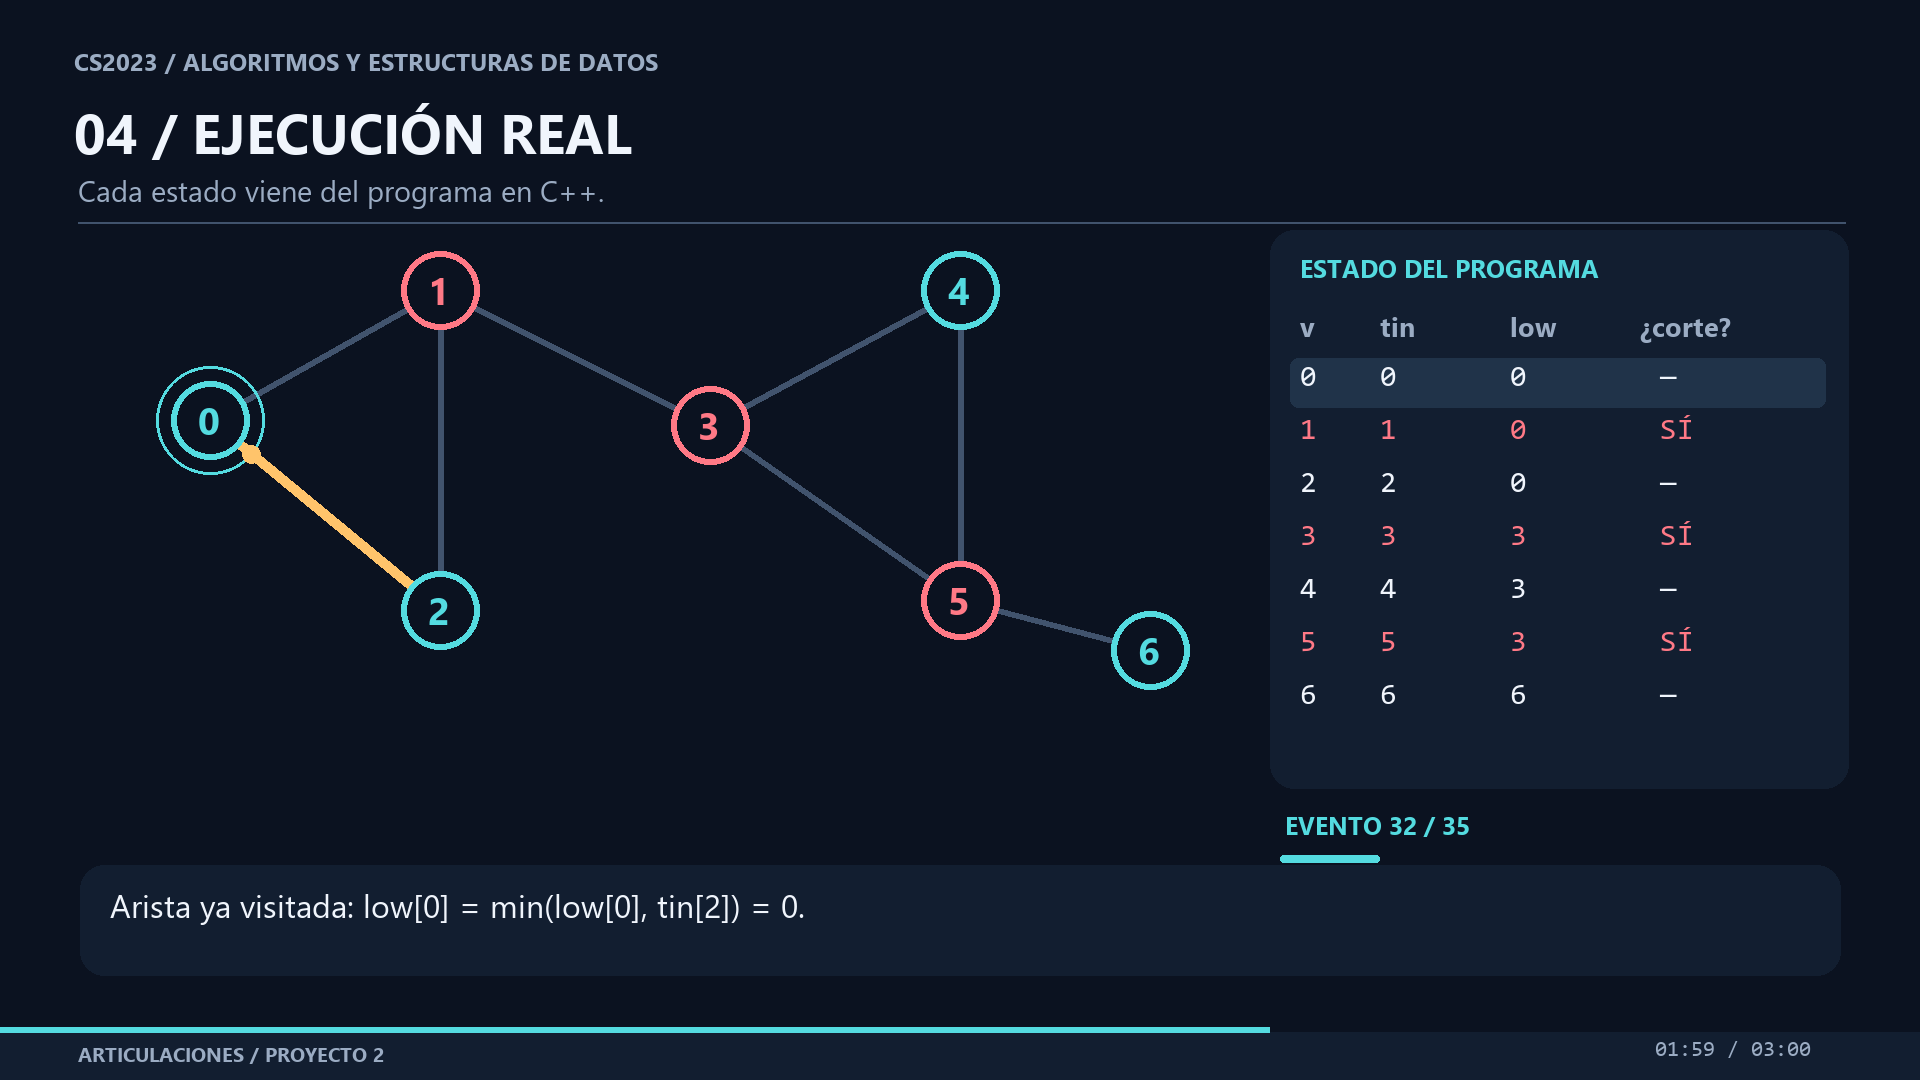
\includegraphics[width=0.48\textwidth]{figuras/ejecucion.png}\hfill
  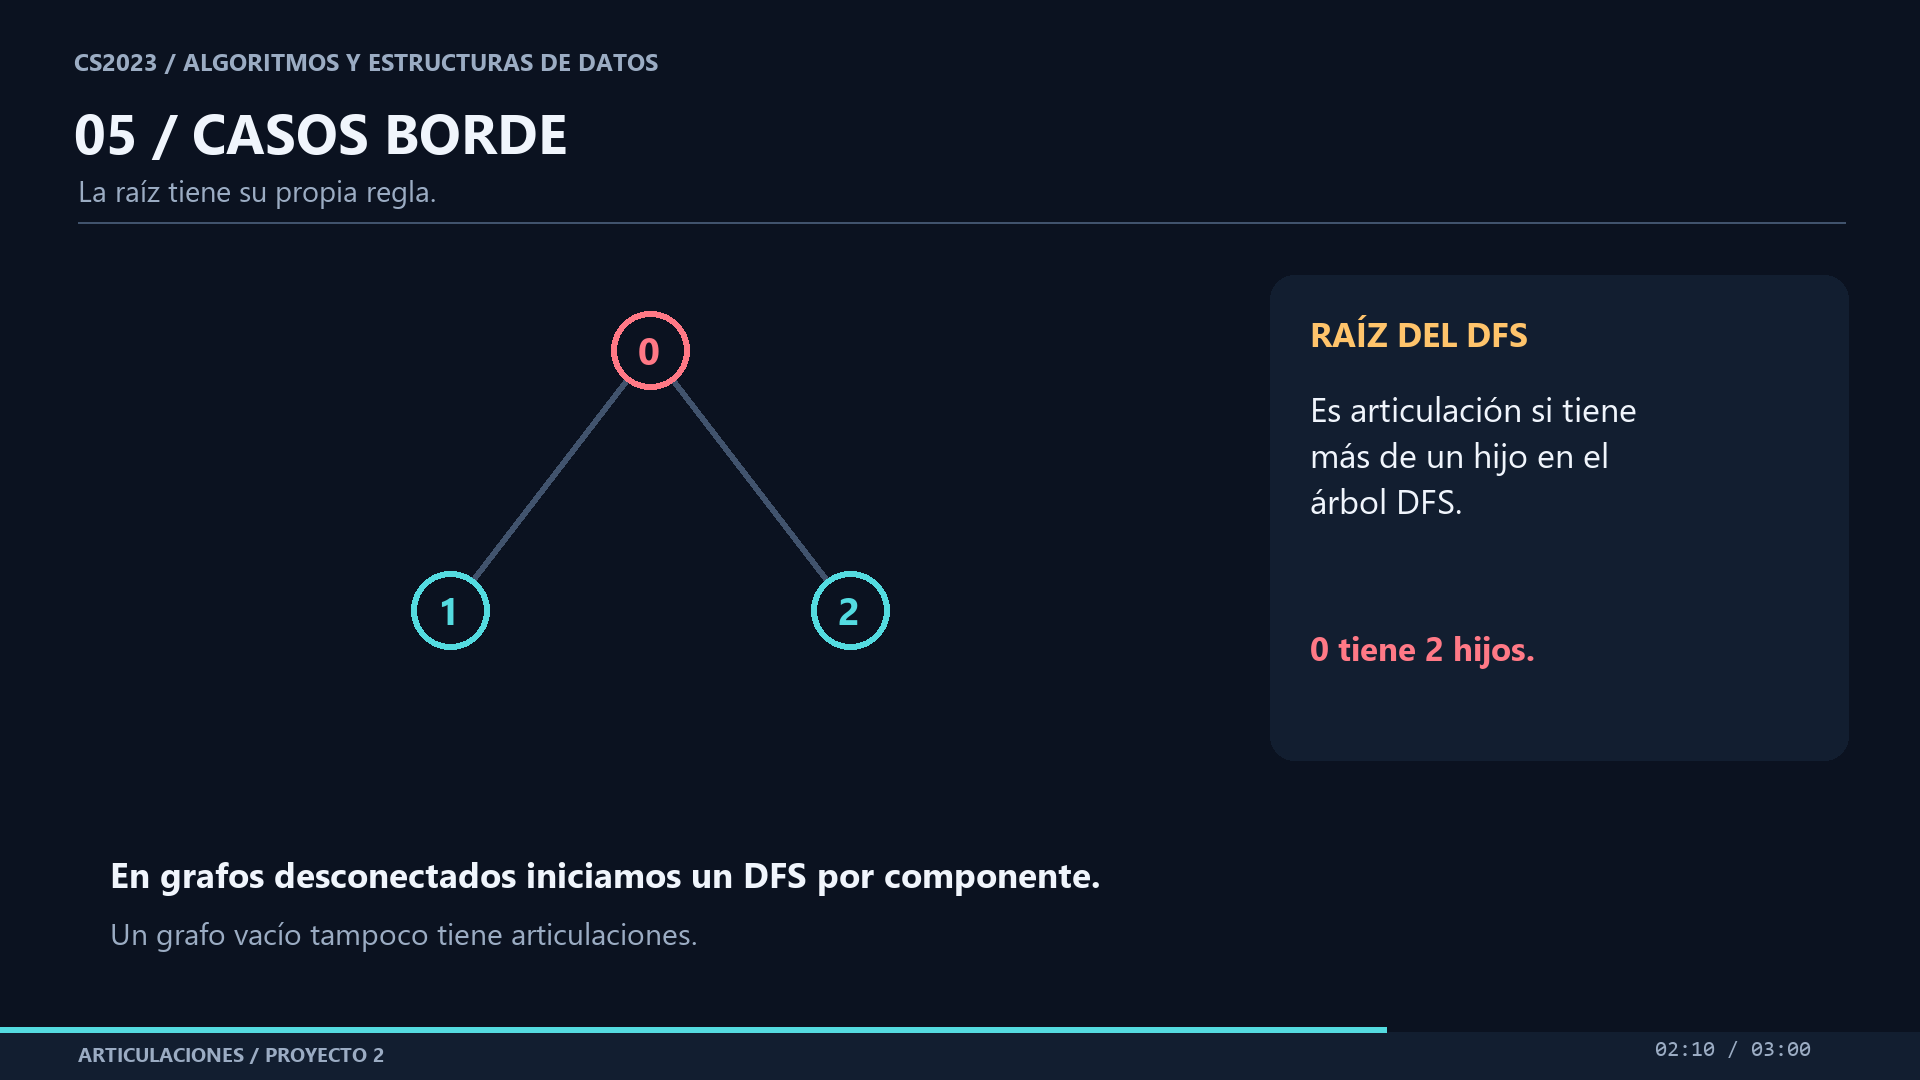
\includegraphics[width=0.48\textwidth]{figuras/raiz.png}
  \caption{Capturas reales generadas por \texttt{proyecto.py --prepare} a
  partir de \texttt{trazas.json}: ejecución sobre \texttt{principal.txt}
  (izquierda) y caso borde de raíz con dos hijos DFS (derecha).}
  \label{fig:evidencias}
\end{figure}

\section{Conclusiones}
\begin{enumerate}
  \item Mantener los tiempos \texttt{tin} y \texttt{low} en un único recorrido
    DFS permite detectar todas las articulaciones en tiempo lineal
    $O(|V|+|E|)$, frente a la estrategia ingenua de eliminar cada vértice y
    recontar componentes en $O(|V|(|V|+|E|))$.
  \item Distinguir entre el caso general ($\texttt{low}[\texttt{to}] \ge
    \texttt{tin}[v]$) y la regla de la raíz (más de un hijo en el árbol DFS),
    junto con la identificación individual de aristas, evita falsos positivos
    en ciclos con raíz y garantiza exactitud ante lazos y aristas paralelas.
  \item Desacoplar el motor en C++17 del renderizado en Python mediante un
    archivo de trazas validado (\texttt{trazas.json}) asegura que la animación
    refleje exactamente los estados calculados por el algoritmo real.
\end{enumerate}

\section*{Referencias}
\begin{itemize}
  \item CS2023, \emph{Proyecto Final 2 -- Anima tu Algoritmo o Estructura de
    Datos}, UTEC, 2026-2 (enunciado entregado por el curso).
  \item \href{https://cp-algorithms.com/graph/cutpoints.html}{CP-Algorithms ---
    Finding articulation points in a graph in $O(N+M)$}, referencia conceptual
    de DFS, valores \texttt{low} y regla de la raíz.
  \item \href{https://pillow.readthedocs.io/}{Documentación oficial de Pillow}
    (generación programática de fotogramas).
  \item \href{https://ffmpeg.org/documentation.html}{Documentación oficial de
    FFmpeg} (codificación H.264 y mezcla de audio).
  \item \href{https://www.3blue1brown.com/}{3Blue1Brown}, referencia de estilo
    visual sugerida en el enunciado del curso.
\end{itemize}

\end{document}
